\section{Results}
\label{sec:results}

\subsection{Preference agreement}
Table~\ref{tab:agree} is the primary result.
Each cell is pairwise accuracy $A$, the effect $A-0.5$, Cohen's $h$, and a Holm-adjusted prompt-cluster $p$.
The bootstrap resamples prompts, not pairs.
Figure~\ref{fig:radar} plots the same point estimates of $A$.
The naive composite is not in this table.
On HPDv2 tattoo-subject pairs, seven pre-registered probes have bootstrap intervals entirely below one half, and those seven remain significant after Holm ($p_{\mathrm{Holm}}\le\HpdFractightgapfivePholm$).
The tight-gap fraction agrees on \HpdFractightgapfiveAcc\ of pairs (effect \HpdFractightgapfiveEffect, $h{=}\HpdFractightgapfiveH$, \HpdFractightgapfiveLo\ to \HpdFractightgapfiveHi, $n{=}\HpdFractightgapfiveN$).
Edge density is \HpdEdgedensitypermmfiveAcc, specks \HpdSpeckspercmfiveAcc, mid-tone fraction \HpdMidtonefracfiveAcc, border variation \HpdBorderstdfiveAcc, sub-needle fraction \HpdFracsubneedlefiveAcc, and minimum line width \HpdLinewpmmfiveAcc.
Open ends are near chance at \HpdOpenendspercmfiveAcc\ (\HpdOpenendspercmfiveLo\ to \HpdOpenendspercmfiveHi).
Post-hoc edge transition is \HpdEdgetransitionmmfiveAcc\ and was not a registered test.
Annotators preferred the image the probes call harder to tattoo.

HPSv2.1 matches the human winner on \HpdHpstwoAcc\ (effect \HpdHpstwoEffect, $h{=}\HpdHpstwoH$, $p_{\mathrm{Holm}}\le\HpdHpstwoPholm$, \HpdHpstwoLo\ to \HpdHpstwoHi, $n{=}\HpdHpstwoN$).
PickScore matches on \HpdPickscoreAcc, CLIPScore on \HpdClipscoreAcc, and ImageReward on \HpdImagerewardAcc.
HPSv2.1 was trained on HPDv2, so that row is in-distribution.
It shows the scorer still ranks these pairs as the annotators did.
It does not show a needle model.

On ImageRewardDB the probes sit near one half, on \NIrTsprompts\ prompts, and none of the \NIrTests\ scorers is significant after Holm (\NIrSigholm).
Tight-gap accuracy is \IrFractightgapfiveAcc\ (effect \IrFractightgapfiveEffect, $h{=}\IrFractightgapfiveH$, \IrFractightgapfiveLo\ to \IrFractightgapfiveHi, $n{=}\IrFractightgapfiveN$, $p_{\mathrm{Holm}}{=}\IrFractightgapfivePholm$).
Mid-tone fraction is the highest probe at \IrMidtonefracfiveAcc.
Edge density is the lowest at \IrEdgedensitypermmfiveAcc.
ImageReward scores \IrImagerewardAcc\ (\IrImagerewardLo\ to \IrImagerewardHi) and was trained on this dataset.
HPSv2.1 is \IrHpstwoAcc\ (\IrHpstwoLo\ to \IrHpstwoHi), PickScore \IrPickscoreAcc, CLIPScore \IrClipscoreAcc.
These intervals are too wide to rank models.

On the Pick-a-Pic tattoo-subject slice the pre-registered probes do not repeat the HPDv2 pattern as a stable ranking.
Tight-gap accuracy is \PapFractightgapfiveAcc\ (\PapFractightgapfiveLo\ to \PapFractightgapfiveHi, $n{=}\PapFractightgapfiveN$), edge density \PapEdgedensitypermmfiveAcc, specks \PapSpeckspercmfiveAcc, mid-tone fraction \PapMidtonefracfiveAcc, and minimum line width \PapLinewpmmfiveAcc.
The intervals cover both sides of one half because there are only \NPapTsprompts\ prompts, and no probe is Holm-significant.
The one Holm-significant scorer on this slice is PickScore (\NPapSigholm\ of \NPapTests, $p_{\mathrm{Holm}}\le\PapPickscorePholm$).
HPSv2.1 matches on \PapHpstwoAcc\ (\PapHpstwoLo\ to \PapHpstwoHi) and ImageReward on \PapImagerewardAcc\ (\PapImagerewardLo\ to \PapImagerewardHi).
Neither model was trained on Pick-a-Pic.
PickScore matches on \PapPickscoreAcc\ and was trained on Pick-a-Pic v1, so that cell is leaky.
CLIPScore is \PapClipscoreAcc.

\begin{figure}[htbp]
  \centering
  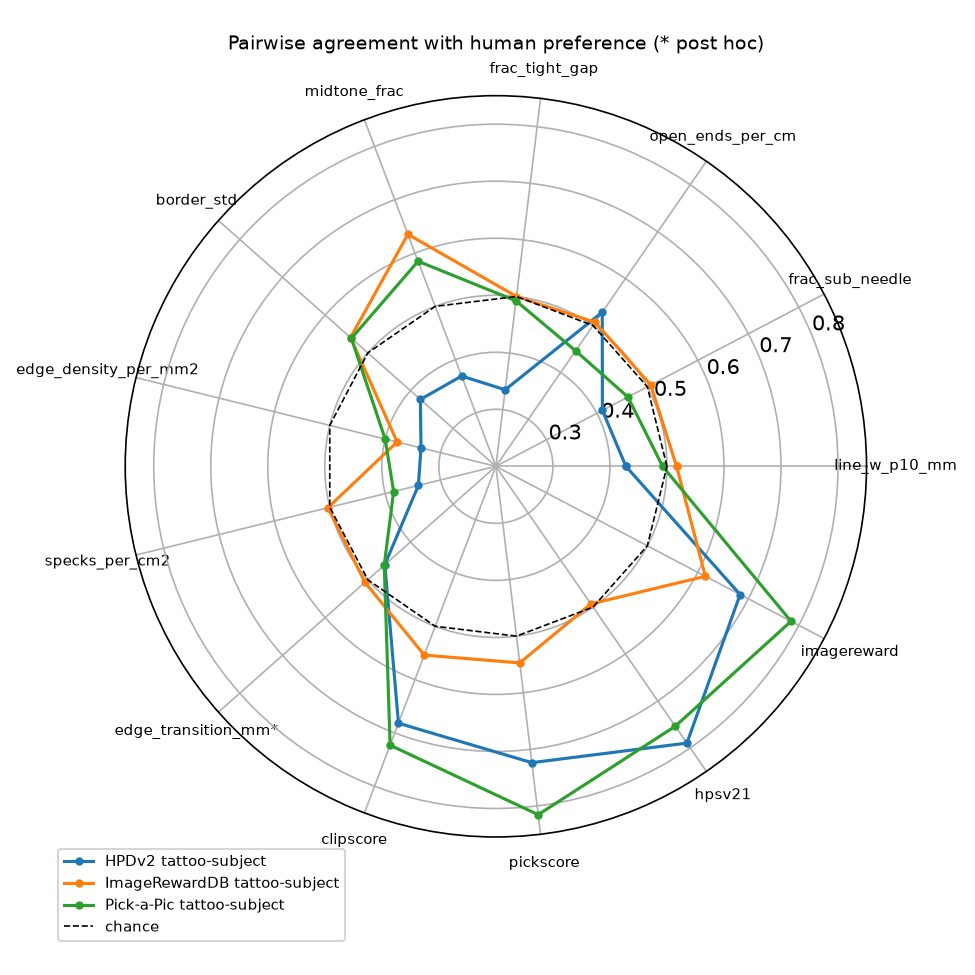
\includegraphics[width=0.48\linewidth]{figures/radar_per_dimension.png}
  \caption{Per-dimension agreement with human preference on the three tattoo-subject slices. Each spoke is one scorer. This is the same comparison as Table~\ref{tab:agree}, without the deprecated composite.}
  \label{fig:radar}
\end{figure}

% auto-generated by tables/make_tables.py
\begin{table}[t]
\centering
\caption{Pairwise accuracy $A$ against human preference on tattoo-subject pairs, the effect $A-0.5$, and Cohen's $h$ against $0.5$. The resampling unit is the prompt (cluster bootstrap, 2000 resamples, seed 0). $p_{\mathrm{Holm}}$ is a two-sided bootstrap $p$ after Holm correction within each dataset across all \NHpdTests\ scorers (the same count on each set: \NIrTests\ and \NPapTests). A printed floor means $p_{\mathrm{Holm}}\le$ that value, which is the bootstrap resolution. Holm-significant scorers: \NHpdSigholm/\NHpdTests\ on HPDv2, \NIrSigholm/\NIrTests\ on ImageRewardDB, \NPapSigholm/\NPapTests\ on Pick-a-Pic. Pair counts are \HpdHpstwoN, \IrHpstwoN\ and \PapHpstwoN. Edge transition is post hoc. HPSv2.1$\leftarrow$HPDv2, ImageReward$\leftarrow$ImageRewardDB and PickScore$\leftarrow$Pick-a-Pic v1 are in-distribution.}
\label{tab:agree}
\resizebox{\linewidth}{!}{%
\footnotesize
\begin{tabular}{lcccccccccccc}
\toprule
& \multicolumn{4}{c}{HPDv2} & \multicolumn{4}{c}{ImageRewardDB} & \multicolumn{4}{c}{Pick-a-Pic} \\
\cmidrule(lr){2-5}\cmidrule(lr){6-9}\cmidrule(lr){10-13}
Scorer & $A$ & $A{-}0.5$ & $h$ & $p_{\mathrm{Holm}}$ & $A$ & $A{-}0.5$ & $h$ & $p_{\mathrm{Holm}}$ & $A$ & $A{-}0.5$ & $h$ & $p_{\mathrm{Holm}}$ \\
\midrule
line\_w p10 & \HpdLinewpmmfiveAcc & \HpdLinewpmmfiveEffect & \HpdLinewpmmfiveH & \HpdLinewpmmfivePholm & \IrLinewpmmfiveAcc & \IrLinewpmmfiveEffect & \IrLinewpmmfiveH & \IrLinewpmmfivePholm & \PapLinewpmmfiveAcc & \PapLinewpmmfiveEffect & \PapLinewpmmfiveH & \PapLinewpmmfivePholm \\
frac sub-needle & \HpdFracsubneedlefiveAcc & \HpdFracsubneedlefiveEffect & \HpdFracsubneedlefiveH & \HpdFracsubneedlefivePholm & \IrFracsubneedlefiveAcc & \IrFracsubneedlefiveEffect & \IrFracsubneedlefiveH & \IrFracsubneedlefivePholm & \PapFracsubneedlefiveAcc & \PapFracsubneedlefiveEffect & \PapFracsubneedlefiveH & \PapFracsubneedlefivePholm \\
open ends / cm & \HpdOpenendspercmfiveAcc & \HpdOpenendspercmfiveEffect & \HpdOpenendspercmfiveH & \HpdOpenendspercmfivePholm & \IrOpenendspercmfiveAcc & \IrOpenendspercmfiveEffect & \IrOpenendspercmfiveH & \IrOpenendspercmfivePholm & \PapOpenendspercmfiveAcc & \PapOpenendspercmfiveEffect & \PapOpenendspercmfiveH & \PapOpenendspercmfivePholm \\
frac tight gap & \HpdFractightgapfiveAcc & \HpdFractightgapfiveEffect & \HpdFractightgapfiveH & \HpdFractightgapfivePholm & \IrFractightgapfiveAcc & \IrFractightgapfiveEffect & \IrFractightgapfiveH & \IrFractightgapfivePholm & \PapFractightgapfiveAcc & \PapFractightgapfiveEffect & \PapFractightgapfiveH & \PapFractightgapfivePholm \\
mid-tone frac. & \HpdMidtonefracfiveAcc & \HpdMidtonefracfiveEffect & \HpdMidtonefracfiveH & \HpdMidtonefracfivePholm & \IrMidtonefracfiveAcc & \IrMidtonefracfiveEffect & \IrMidtonefracfiveH & \IrMidtonefracfivePholm & \PapMidtonefracfiveAcc & \PapMidtonefracfiveEffect & \PapMidtonefracfiveH & \PapMidtonefracfivePholm \\
border std & \HpdBorderstdfiveAcc & \HpdBorderstdfiveEffect & \HpdBorderstdfiveH & \HpdBorderstdfivePholm & \IrBorderstdfiveAcc & \IrBorderstdfiveEffect & \IrBorderstdfiveH & \IrBorderstdfivePholm & \PapBorderstdfiveAcc & \PapBorderstdfiveEffect & \PapBorderstdfiveH & \PapBorderstdfivePholm \\
edge density & \HpdEdgedensitypermmfiveAcc & \HpdEdgedensitypermmfiveEffect & \HpdEdgedensitypermmfiveH & \HpdEdgedensitypermmfivePholm & \IrEdgedensitypermmfiveAcc & \IrEdgedensitypermmfiveEffect & \IrEdgedensitypermmfiveH & \IrEdgedensitypermmfivePholm & \PapEdgedensitypermmfiveAcc & \PapEdgedensitypermmfiveEffect & \PapEdgedensitypermmfiveH & \PapEdgedensitypermmfivePholm \\
specks / cm$^2$ & \HpdSpeckspercmfiveAcc & \HpdSpeckspercmfiveEffect & \HpdSpeckspercmfiveH & \HpdSpeckspercmfivePholm & \IrSpeckspercmfiveAcc & \IrSpeckspercmfiveEffect & \IrSpeckspercmfiveH & \IrSpeckspercmfivePholm & \PapSpeckspercmfiveAcc & \PapSpeckspercmfiveEffect & \PapSpeckspercmfiveH & \PapSpeckspercmfivePholm \\
edge transition & \HpdEdgetransitionmmfiveAcc & \HpdEdgetransitionmmfiveEffect & \HpdEdgetransitionmmfiveH & \HpdEdgetransitionmmfivePholm & \IrEdgetransitionmmfiveAcc & \IrEdgetransitionmmfiveEffect & \IrEdgetransitionmmfiveH & \IrEdgetransitionmmfivePholm & \PapEdgetransitionmmfiveAcc & \PapEdgetransitionmmfiveEffect & \PapEdgetransitionmmfiveH & \PapEdgetransitionmmfivePholm \\
CLIPScore & \HpdClipscoreAcc & \HpdClipscoreEffect & \HpdClipscoreH & \HpdClipscorePholm & \IrClipscoreAcc & \IrClipscoreEffect & \IrClipscoreH & \IrClipscorePholm & \PapClipscoreAcc & \PapClipscoreEffect & \PapClipscoreH & \PapClipscorePholm \\
PickScore & \HpdPickscoreAcc & \HpdPickscoreEffect & \HpdPickscoreH & \HpdPickscorePholm & \IrPickscoreAcc & \IrPickscoreEffect & \IrPickscoreH & \IrPickscorePholm & \PapPickscoreAcc & \PapPickscoreEffect & \PapPickscoreH & \PapPickscorePholm \\
HPSv2.1 & \HpdHpstwoAcc & \HpdHpstwoEffect & \HpdHpstwoH & \HpdHpstwoPholm & \IrHpstwoAcc & \IrHpstwoEffect & \IrHpstwoH & \IrHpstwoPholm & \PapHpstwoAcc & \PapHpstwoEffect & \PapHpstwoH & \PapHpstwoPholm \\
ImageReward & \HpdImagerewardAcc & \HpdImagerewardEffect & \HpdImagerewardH & \HpdImagerewardPholm & \IrImagerewardAcc & \IrImagerewardEffect & \IrImagerewardH & \IrImagerewardPholm & \PapImagerewardAcc & \PapImagerewardEffect & \PapImagerewardH & \PapImagerewardPholm \\
\bottomrule
\end{tabular}}
\end{table}


\subsection{Fusion learns the opposite signs}
A prompt-held-out logistic fusion of the eight pre-registered probes reaches \FusHpdProbespreregisteredAcc\ on HPDv2 (\FusHpdProbespreregisteredLo\ to \FusHpdProbespreregisteredHi, $n{=}\FusHpdProbespreregisteredN$).
Adding edge transition leaves \FusHpdProbesallAcc.
The full-sample coefficients invert the a-priori signs for line width, sub-needle fraction, tight gaps, mid-tones, border variation, edge density and specks.
Only open ends stay negative.
The fusion predicts annotator taste by rewarding features the probes call worse to tattoo.
Reward fusion reaches \FusHpdRewardsAcc\ ($n{=}\FusHpdRewardsN$) and is not improved by adding probes (\FusHpdRewardsprobesAcc).
In the reward-only fit the HPSv2.1 coefficient is positive and dominates; PickScore's coefficient is negative.

On ImageRewardDB the pre-registered probe fusion is \FusIrProbespreregisteredAcc\ (\FusIrProbespreregisteredLo\ to \FusIrProbespreregisteredHi).
Reward fusion is \FusIrRewardsAcc; adding probes lowers it to \FusIrRewardsprobesAcc.
The reward-only fit puts a positive sign on ImageReward and a negative sign on HPSv2.1.
We do not treat the probe signs on \NIrTsprompts\ prompts as stable.

On Pick-a-Pic the pre-registered probe fusion is \FusPapProbespreregisteredAcc\ (\FusPapProbespreregisteredLo\ to \FusPapProbespreregisteredHi, $n{=}\FusPapProbespreregisteredN$), below one half, and the all-probe fusion is \FusPapProbesallAcc.
The full-sample signs are not the HPDv2 inversion.
Line width is negative, and edge density and specks are positive, so those three disagree with the a-priori tattooability signs.
Sub-needle fraction, open ends, tight gaps, mid-tones and border variation keep the a-priori sign.
Reward fusion reaches \FusPapRewardsAcc\ (\FusPapRewardsLo\ to \FusPapRewardsHi); adding probes lowers it to \FusPapRewardsprobesAcc.
In the reward-only fit PickScore and ImageReward are positive and HPSv2.1 is negative.
The PickScore term is the leaky one.

% auto-generated by tables/make_tables.py
\begin{table}[t]
\centering
\caption{Prompt-held-out logistic fusion (GroupKFold on prompt, $k{=}5$, seed 0). Accuracy is the fraction of pairs whose held-out predicted winner matches the human winner. Brackets are 95\% prompt-cluster bootstrap intervals (2000 resamples). Coefficient signs are discussed in the text; magnitudes stay in \texttt{fusion\_lopo.csv}. On Pick-a-Pic the reward fusion is led by PickScore, which was trained on Pick-a-Pic v1.}
\label{tab:fusion}
\resizebox{\linewidth}{!}{%
\footnotesize
\begin{tabular}{lcccccc}
\toprule
Model & HPDv2 acc. [CI] & $n$ & ImageRewardDB acc. [CI] & $n$ & Pick-a-Pic acc. [CI] & $n$ \\
\midrule
Probes, pre-registered & \FusHpdProbespreregisteredAcc\ [\FusHpdProbespreregisteredLo, \FusHpdProbespreregisteredHi] & \FusHpdProbespreregisteredN & \FusIrProbespreregisteredAcc\ [\FusIrProbespreregisteredLo, \FusIrProbespreregisteredHi] & \FusIrProbespreregisteredN & \FusPapProbespreregisteredAcc\ [\FusPapProbespreregisteredLo, \FusPapProbespreregisteredHi] & \FusPapProbespreregisteredN \\
Probes, including edge transition & \FusHpdProbesallAcc\ [\FusHpdProbesallLo, \FusHpdProbesallHi] & \FusHpdProbesallN & \FusIrProbesallAcc\ [\FusIrProbesallLo, \FusIrProbesallHi] & \FusIrProbesallN & \FusPapProbesallAcc\ [\FusPapProbesallLo, \FusPapProbesallHi] & \FusPapProbesallN \\
Rewards & \FusHpdRewardsAcc\ [\FusHpdRewardsLo, \FusHpdRewardsHi] & \FusHpdRewardsN & \FusIrRewardsAcc\ [\FusIrRewardsLo, \FusIrRewardsHi] & \FusIrRewardsN & \FusPapRewardsAcc\ [\FusPapRewardsLo, \FusPapRewardsHi] & \FusPapRewardsN \\
Rewards + all probes & \FusHpdRewardsprobesAcc\ [\FusHpdRewardsprobesLo, \FusHpdRewardsprobesHi] & \FusHpdRewardsprobesN & \FusIrRewardsprobesAcc\ [\FusIrRewardsprobesLo, \FusIrRewardsprobesHi] & \FusIrRewardsprobesN & \FusPapRewardsprobesAcc\ [\FusPapRewardsprobesLo, \FusPapRewardsprobesHi] & \FusPapRewardsprobesN \\
\bottomrule
\end{tabular}}
\end{table}


\subsection{Injected defects}
Table~\ref{tab:degr} asks whether a known damage lowers the score.
At 5\,cm, edge transition rates blur at \DgEdgetransitionmmfiveBlurOne\ and \DgEdgetransitionmmfiveBlurTwo, detail loss at \DgEdgetransitionmmfiveDetaillossOne\ and \DgEdgetransitionmmfiveDetaillossTwo, and thickening at \DgEdgetransitionmmfiveThickenOne\ and \DgEdgetransitionmmfiveThickenTwo.
Mid-tone fraction rates haze at \DgMidtonefracfiveHazeOne\ and speckle at \DgMidtonefracfiveSpeckleOne.
Sub-needle fraction rates thinning at \DgFracsubneedlefiveThinOne\ and \DgFracsubneedlefiveThinTwo.
The deprecated composite is omitted here and stated once in Appendix~\ref{app:probes}.

HPSv2.1's lowest cell in the table is light blur at \DgHpstwoBlurOne.
PickScore on that cell is \DgPickscoreBlurOne.
CLIPScore on speckle is \DgClipscoreSpeckleOne\ and \DgClipscoreSpeckleTwo.
ImageReward on heavy speckle is \DgImagerewardSpeckleTwo.
Rewards detect many defects and do not name the millimetre quantity that moved.
Figure~\ref{fig:degr} shows the grid.

% auto-generated by tables/make_tables.py
\begin{table}[t]
\centering
\caption{Controlled-defect detection at a 5\,cm print size: fraction of designs on which the clean image scores better than the degraded image (ties count as one half). Probe columns use a-priori signs. Reward columns use the raw reward (higher is better). The deprecated composite is not a column here; Appendix~\ref{app:probes} states it in one sentence. $n{=}\nDegrRewDesigns$ designs per cell (the reward subset).}
\label{tab:degr}
\resizebox{\linewidth}{!}{%
\footnotesize
\begin{tabular}{llcccccccc}
\toprule
Defect & Lv. & trans. & sub-ndl & gap & mid & HPS & IR & Pick & CLIP \\
\midrule
blur & 1 & \DgEdgetransitionmmfiveBlurOne & \DgFracsubneedlefiveBlurOne & \DgFractightgapfiveBlurOne & \DgMidtonefracfiveBlurOne & \DgHpstwoBlurOne & \DgImagerewardBlurOne & \DgPickscoreBlurOne & \DgClipscoreBlurOne \\
blur & 2 & \DgEdgetransitionmmfiveBlurTwo & \DgFracsubneedlefiveBlurTwo & \DgFractightgapfiveBlurTwo & \DgMidtonefracfiveBlurTwo & \DgHpstwoBlurTwo & \DgImagerewardBlurTwo & \DgPickscoreBlurTwo & \DgClipscoreBlurTwo \\
detail loss & 1 & \DgEdgetransitionmmfiveDetaillossOne & \DgFracsubneedlefiveDetaillossOne & \DgFractightgapfiveDetaillossOne & \DgMidtonefracfiveDetaillossOne & \DgHpstwoDetaillossOne & \DgImagerewardDetaillossOne & \DgPickscoreDetaillossOne & \DgClipscoreDetaillossOne \\
detail loss & 2 & \DgEdgetransitionmmfiveDetaillossTwo & \DgFracsubneedlefiveDetaillossTwo & \DgFractightgapfiveDetaillossTwo & \DgMidtonefracfiveDetaillossTwo & \DgHpstwoDetaillossTwo & \DgImagerewardDetaillossTwo & \DgPickscoreDetaillossTwo & \DgClipscoreDetaillossTwo \\
haze & 1 & \DgEdgetransitionmmfiveHazeOne & \DgFracsubneedlefiveHazeOne & \DgFractightgapfiveHazeOne & \DgMidtonefracfiveHazeOne & \DgHpstwoHazeOne & \DgImagerewardHazeOne & \DgPickscoreHazeOne & \DgClipscoreHazeOne \\
haze & 2 & \DgEdgetransitionmmfiveHazeTwo & \DgFracsubneedlefiveHazeTwo & \DgFractightgapfiveHazeTwo & \DgMidtonefracfiveHazeTwo & \DgHpstwoHazeTwo & \DgImagerewardHazeTwo & \DgPickscoreHazeTwo & \DgClipscoreHazeTwo \\
speckle & 1 & \DgEdgetransitionmmfiveSpeckleOne & \DgFracsubneedlefiveSpeckleOne & \DgFractightgapfiveSpeckleOne & \DgMidtonefracfiveSpeckleOne & \DgHpstwoSpeckleOne & \DgImagerewardSpeckleOne & \DgPickscoreSpeckleOne & \DgClipscoreSpeckleOne \\
speckle & 2 & \DgEdgetransitionmmfiveSpeckleTwo & \DgFracsubneedlefiveSpeckleTwo & \DgFractightgapfiveSpeckleTwo & \DgMidtonefracfiveSpeckleTwo & \DgHpstwoSpeckleTwo & \DgImagerewardSpeckleTwo & \DgPickscoreSpeckleTwo & \DgClipscoreSpeckleTwo \\
thicken & 1 & \DgEdgetransitionmmfiveThickenOne & \DgFracsubneedlefiveThickenOne & \DgFractightgapfiveThickenOne & \DgMidtonefracfiveThickenOne & \DgHpstwoThickenOne & \DgImagerewardThickenOne & \DgPickscoreThickenOne & \DgClipscoreThickenOne \\
thicken & 2 & \DgEdgetransitionmmfiveThickenTwo & \DgFracsubneedlefiveThickenTwo & \DgFractightgapfiveThickenTwo & \DgMidtonefracfiveThickenTwo & \DgHpstwoThickenTwo & \DgImagerewardThickenTwo & \DgPickscoreThickenTwo & \DgClipscoreThickenTwo \\
thin & 1 & \DgEdgetransitionmmfiveThinOne & \DgFracsubneedlefiveThinOne & \DgFractightgapfiveThinOne & \DgMidtonefracfiveThinOne & \DgHpstwoThinOne & \DgImagerewardThinOne & \DgPickscoreThinOne & \DgClipscoreThinOne \\
thin & 2 & \DgEdgetransitionmmfiveThinTwo & \DgFracsubneedlefiveThinTwo & \DgFractightgapfiveThinTwo & \DgMidtonefracfiveThinTwo & \DgHpstwoThinTwo & \DgImagerewardThinTwo & \DgPickscoreThinTwo & \DgClipscoreThinTwo \\
\bottomrule
\end{tabular}}
\end{table}


\begin{figure}[htbp]
  \centering
  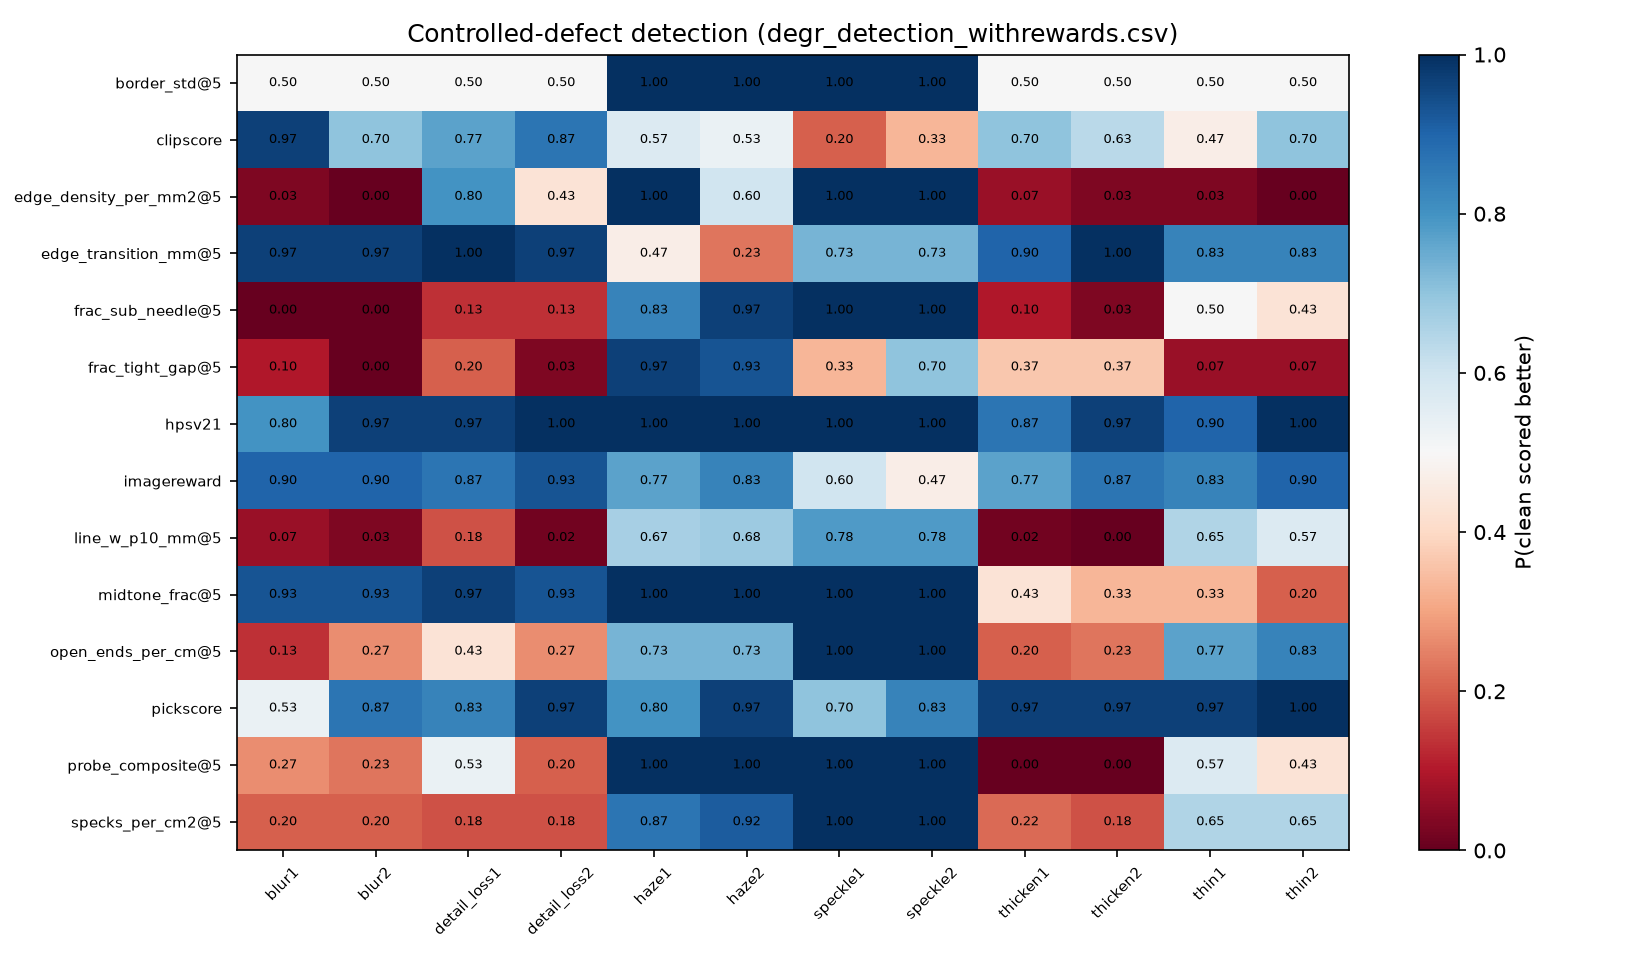
\includegraphics[width=0.55\linewidth]{figures/degr_detection.png}
  \caption{Detection rates on six injected defects at two strengths. The 5\,cm numbers for the probes we interpret, and for the four rewards, are in Table~\ref{tab:degr}.}
  \label{fig:degr}
\end{figure}

\subsection{Scale and spread}
With no additive pixel noise, skeleton $F_1$ at spread $\sigma{=}0$ is \ssFoneSizeThreeSpreadZero\ at $s{=}3$\,cm, \ssFoneSizeFiveSpreadZero\ at $s{=}5$\,cm, \ssFoneSizeTenSpreadZero\ at $s{=}10$\,cm and \ssFoneSizeFifteenSpreadZero\ at $s{=}15$\,cm (Table~\ref{tab:scale}, Figure~\ref{fig:scale}).
The same four sizes under the old $\sigma{=}4$ grey-level noise are \ssNoiseFoneThree, \ssNoiseFoneFive, \ssNoiseFoneTen\ and \ssNoiseFoneFifteen, which fall as the print grows.
That fall is not in the default grid.
At 0.30\,mm spread, default $F_1$ is \ssFoneSizeThreeSpreadThirty, \ssFoneSizeFiveSpreadThirty, \ssFoneSizeTenSpreadThirty\ and \ssFoneSizeFifteenSpreadThirty.
At 0.60\,mm it is \ssFoneSizeThreeSpreadSixty, \ssFoneSizeFiveSpreadSixty, \ssFoneSizeTenSpreadSixty\ and \ssFoneSizeFifteenSpreadSixty.
Gap survival at 0.30\,mm is \ssGapSizeThreeSpreadThirty, \ssGapSizeFiveSpreadThirty, \ssGapSizeTenSpreadThirty\ and \ssGapSizeFifteenSpreadThirty.
Table~\ref{tab:scale} reports a subset of that 0.05\,mm grid.

Table~\ref{tab:minsize} is the size at which mean skeleton $F_1$ first reaches seven tenths, and eight tenths.
At zero spread both levels are met at \minSizeSeventySpreadZero\,cm.
At 0.20\,mm the seven-tenths size is \minSizeSeventySpreadTwenty\,cm and the eight-tenths size is \minSizeEightySpreadTwenty\,cm.
At 0.30\,mm the seven-tenths size is \minSizeSeventySpreadThirty\,cm and eight tenths is \minSizeEightySpreadThirty.
At 0.60\,mm neither level is reached (\minSizeSeventySpreadSixty, \minSizeEightySpreadSixty).

At 5\,cm and 0.30\,mm, tight-gap fraction correlates with gap survival at \RhoFractightgapGapsurvival\ (partly circular), edge density with gap survival at \RhoEdgedensitypermmGapsurvival, edge transition with skeleton $F_1$ at \RhoEdgetransitionmmSkelf, and minimum line width with skeleton $F_1$ at \RhoLinewpmmSkelf.
These associations live inside the simulator.

\begin{figure}[htbp]
  \centering
  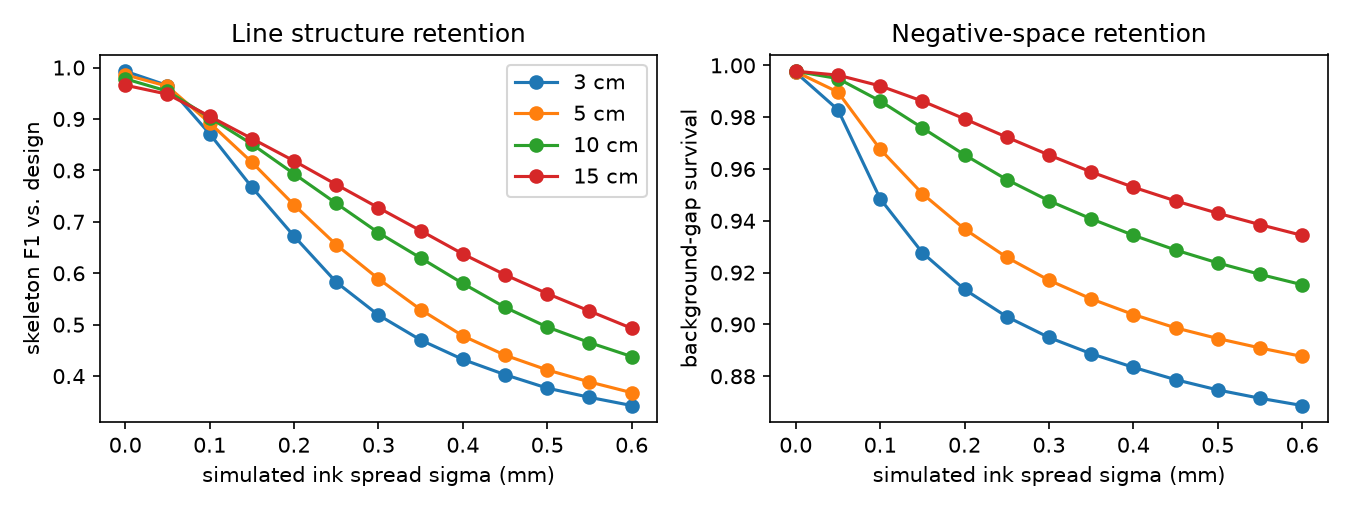
\includegraphics[width=0.72\linewidth]{figures/scale_spread.png}
  \caption{Mean skeleton $F_1$ against ink spread $\sigma$ at each print size $s$. The grid is the default simulator: no additive pixel noise. Table~\ref{tab:scale} lists a subset of the same cells.}
  \label{fig:scale}
\end{figure}

% auto-generated by tables/make_tables.py
\begin{table}[t]
\centering
\caption{Mean skeleton $F_1$ (tolerance 0.2\,mm) and, on the following row, mean gap survival. Default simulation: no additive pixel noise, and the same Otsu threshold on the reference and the blurred image. Rows are longest-side print sizes in centimetres. Columns are a subset of the 0 to 0.60\,mm grid (step 0.05\,mm); the figure shows every step. Each cell averages \nDegrDesigns\ designs. At spread 0, $F_1$ is exact on this grid.}
\label{tab:scale}
\resizebox{\linewidth}{!}{%
\footnotesize
\begin{tabular}{lccccc}
\toprule
Size (cm) & 0 & 0.15 & 0.30 & 0.45 & 0.60 \\
\midrule
3 & \ssFoneSizeThreeSpreadZero & \ssFoneSizeThreeSpreadFifteen & \ssFoneSizeThreeSpreadThirty & \ssFoneSizeThreeSpreadFortyFive & \ssFoneSizeThreeSpreadSixty \\
3 (gap) & \ssGapSizeThreeSpreadZero & \ssGapSizeThreeSpreadFifteen & \ssGapSizeThreeSpreadThirty & \ssGapSizeThreeSpreadFortyFive & \ssGapSizeThreeSpreadSixty \\
5 & \ssFoneSizeFiveSpreadZero & \ssFoneSizeFiveSpreadFifteen & \ssFoneSizeFiveSpreadThirty & \ssFoneSizeFiveSpreadFortyFive & \ssFoneSizeFiveSpreadSixty \\
5 (gap) & \ssGapSizeFiveSpreadZero & \ssGapSizeFiveSpreadFifteen & \ssGapSizeFiveSpreadThirty & \ssGapSizeFiveSpreadFortyFive & \ssGapSizeFiveSpreadSixty \\
10 & \ssFoneSizeTenSpreadZero & \ssFoneSizeTenSpreadFifteen & \ssFoneSizeTenSpreadThirty & \ssFoneSizeTenSpreadFortyFive & \ssFoneSizeTenSpreadSixty \\
10 (gap) & \ssGapSizeTenSpreadZero & \ssGapSizeTenSpreadFifteen & \ssGapSizeTenSpreadThirty & \ssGapSizeTenSpreadFortyFive & \ssGapSizeTenSpreadSixty \\
15 & \ssFoneSizeFifteenSpreadZero & \ssFoneSizeFifteenSpreadFifteen & \ssFoneSizeFifteenSpreadThirty & \ssFoneSizeFifteenSpreadFortyFive & \ssFoneSizeFifteenSpreadSixty \\
15 (gap) & \ssGapSizeFifteenSpreadZero & \ssGapSizeFifteenSpreadFifteen & \ssGapSizeFifteenSpreadThirty & \ssGapSizeFifteenSpreadFortyFive & \ssGapSizeFifteenSpreadSixty \\
\bottomrule
\end{tabular}}
\end{table}

% auto-generated by tables/make_tables.py
\begin{table}[t]
\centering
\caption{Smallest tested print size, in centimetres, whose mean skeleton $F_1$ reaches seven tenths or eight tenths at that spread. \texttt{n/a} means no tested size up to 15\,cm reached the level. Noise is off. This is a sensitivity table for the simulator, not a healed-skin recommendation.}
\label{tab:minsize}
\footnotesize
\begin{tabular}{lcc}
\toprule
Spread (mm) & Min.\ size, $F_1$ seven tenths & Min.\ size, $F_1$ eight tenths \\
\midrule
0 & \minSizeSeventySpreadZero & \minSizeEightySpreadZero \\
0.10 & \minSizeSeventySpreadTen & \minSizeEightySpreadTen \\
0.20 & \minSizeSeventySpreadTwenty & \minSizeEightySpreadTwenty \\
0.30 & \minSizeSeventySpreadThirty & \minSizeEightySpreadThirty \\
0.40 & \minSizeSeventySpreadForty & \minSizeEightySpreadForty \\
0.50 & \minSizeSeventySpreadFifty & \minSizeEightySpreadFifty \\
0.60 & \minSizeSeventySpreadSixty & \minSizeEightySpreadSixty \\
\bottomrule
\end{tabular}
\end{table}



